\section{Experiments}
\begin{figure}[t]
\centering
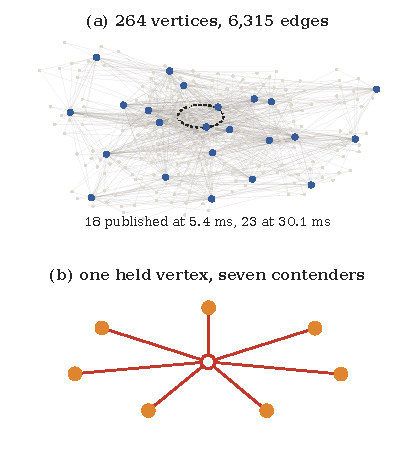
\includegraphics[width=.86\columnwidth]{figures/qualitative_instance.pdf}
\caption{\textbf{One instance, release to delivery.}
(a) Graph index~848 of RB-[200,300] (264 vertices, 6,315 edges). SPRINT-C publishes 18 vertices at 5.4~ms and delivers 23 at 30.1~ms (blue); the dashed circle marks the pocket in (b).
(b) The held vertex~149 conflicts with seven vertices that the final set selects, so none of the seven can join while it is held; exchanges drop such a vertex and admit its contenders. Resident OnlineMIS delivers 22 vertices on this graph at 7.8~ms.}
\label{fig:qualitative-instance}
\end{figure}


\label{sec:experiments}

\paragraph{Instances and protocol.}
The released MIS benchmarks contain 1,000 graphs each in RB-[200--300] and RB-[800--1200], 128 in ER-[700--800], and 16 in ER-[9000--11000] \citep{feng2025regularized}. Solvers are paired on graph ID and search seed (1017, 1019, 1021), giving 6,432 graph--seed pairs per budget, and at each of four budgets every resident solver runs on all pairs from the same host edge list. Table~\ref{tab:external-deadline} collects every measured method at the common 200~ms cutoff. The transfer study uses all 14 register interference graphs in the DIMACS COLOR catalog \citep{johnson1996dimacs}. We report mean delivered size with missed deliveries scored zero, the number of runs with a set on the host, and the actual return time. Paired contrasts average the three differences on each graph and resample graphs 5,000 times; all intervals are pointwise 95\%. Appendix~\ref{app:protocol} specifies training, validation and timing for every implementation.

\subsection{SPRINT-C delivers the largest set at 200 ms}
\begin{table*}[t]
\centering\footnotesize\setlength{\tabcolsep}{2.6pt}
\caption{Maximum independent set at 200\,ms per graph. Size averages the largest feasible set delivered to the host by the cutoff over all $N$ graph--seed pairs. A missed delivery scores zero. Ready counts timely deliveries. Time is the mean wall time per call in milliseconds, including overruns. DiffUCO skips inference on large RB and large ER after calibration. An em dash marks an unavailable measurement (Gurobi license details in Appendix~\ref{app:protocol}). Bold marks the highest mean size in each range.}
\label{tab:external-deadline}
\resizebox{\textwidth}{!}{\begin{tabular}{lrrrrrrrrrrrr}
\toprule
\paperHeader & \multicolumn{3}{c}{\paperHead{RB-[200--300]}} & \multicolumn{3}{c}{\paperHead{RB-[800--1200]}} & \multicolumn{3}{c}{\paperHead{ER-[700--800]}} & \multicolumn{3}{c}{\paperHead{ER-[9000--11000]}} \\
\paperHeader & \multicolumn{3}{c}{$N=3000$} & \multicolumn{3}{c}{$N=3000$} & \multicolumn{3}{c}{$N=384$} & \multicolumn{3}{c}{$N=48$} \\
\cmidrule(lr){2-4}\cmidrule(lr){5-7}\cmidrule(lr){8-10}\cmidrule(lr){11-13}
\paperHeader \paperHead{Solver} & \paperHead{Size\,$\uparrow$} & \paperHead{Time\,$\downarrow$} & \paperHead{Ready} & \paperHead{Size\,$\uparrow$} & \paperHead{Time\,$\downarrow$} & \paperHead{Ready} & \paperHead{Size\,$\uparrow$} & \paperHead{Time\,$\downarrow$} & \paperHead{Ready} & \paperHead{Size\,$\uparrow$} & \paperHead{Time\,$\downarrow$} & \paperHead{Ready} \\
\midrule
Gurobi (vertex MIP) & 16.5967 & 200.61 & 3000 & 32.0680 & 208.14 & 3000 & 29.8984 & 213.29 & 384 & \multicolumn{3}{c}{\textemdash} \\
KaMIS (ReduMIS CLI) & 1.8473 & 195.64 & 280 & 0.3490 & 202.75 & 26 & 0.0000 & 202.90 & 0 & 0.0000 & 206.18 & 0 \\
OnlineMIS (tuned CLI) & 20.0087 & 188.56 & 2994 & 41.6140 & 152.35 & 2997 & 42.5365 & 151.19 & 384 & 0.0000 & 206.15 & 0 \\
\rowcolor{TableOrange}
OnlineMIS (resident) & 20.0817 & 197.11 & 3000 & 41.7613 & 197.72 & 3000 & 42.7240 & 198.00 & 384 & 363.5833 & 197.48 & 48 \\
Released RLNN & 19.4247 & 152.25 & 2999 & 34.7923 & 166.72 & 2993 & 40.5469 & 145.57 & 383 & 0.0000 & 1606.14 & 0 \\
FLD-EG (recon.) & 18.3327 & 183.45 & 2999 & 35.3673 & 182.26 & 2999 & 34.9688 & 179.93 & 383 & 0.0000 & 346.88 & 0 \\
DiffUCO & 19.6473 & 52.22 & 3000 & 0.0000 & $<0.01$ & 0 & 42.8333 & 157.20 & 384 & 0.0000 & $<0.01$ & 0 \\
LTFT & 14.1917 & 191.25 & 3000 & 20.9747 & 195.55 & 3000 & 21.1562 & 198.41 & 383 & 3.7083 & 181.07 & 48 \\
DIFUSCO & 15.3523 & 161.78 & 2997 & 31.7993 & 94.99 & 3000 & 28.7109 & 165.92 & 355 & 0.0000 & 669.41 & 0 \\
DGL-TreeSearch & 5.0850 & 169.55 & 3000 & 6.1747 & 173.49 & 3000 & 9.4531 & 164.76 & 384 & 0.0000 & 25.30 & 0 \\
DIMES (ER retrain) & 18.9183 & 197.54 & 3000 & 35.4367 & 191.76 & 3000 & 37.4297 & 193.35 & 384 & 178.8542 & 279.00 & 30 \\
INTEL & 17.1893 & 200.24 & 3000 & 24.1410 & 200.23 & 3000 & 37.3620 & 201.16 & 384 & 65.6042 & 200.53 & 48 \\
PPO-LwD & 16.0697 & 190.43 & 3000 & 29.5217 & 192.71 & 3000 & 32.1667 & 193.29 & 384 & 208.1875 & 193.09 & 48 \\
DISCS iSCO & 19.3037 & 198.48 & 2960 & 0.1477 & 190.91 & 14 & 40.5677 & 196.05 & 383 & 0.0000 & 183.63 & 0 \\
RLSA & 19.9507 & 156.52 & 2999 & 31.2113 & 166.55 & 2527 & 43.1536 & 167.75 & 383 & 0.0000 & 2011.52 & 0 \\
iSCO (300 steps) & 11.4743 & 104.06 & 1804 & 0.1473 & 190.97 & 14 & 40.6146 & 195.74 & 383 & 0.0000 & 182.09 & 0 \\
\midrule
\rowcolor{TableGreen}
SPRINT-C (degree) & \textbf{20.1150} & 2.53 & 3000 & \textbf{42.4663} & 137.18 & 3000 & 44.2578 & 197.06 & 384 & 369.4167 & 197.27 & 48 \\
\rowcolor{TableBlue}
\textbf{SPRINT-C (learned)} & \textbf{20.1150} & 10.37 & 3000 & 42.4417 & 139.04 & 3000 & \textbf{44.3438} & 197.08 & 384 & \textbf{370.1250} & 197.24 & 48 \\
\bottomrule
\end{tabular}}
\end{table*}

At 200~ms SPRINT-C delivers the largest mean set of every measured solver on all four families (Table~\ref{tab:external-deadline}): 20.1150 against 20.0817 for resident OnlineMIS on small RB ($+0.0333$, $[0.0253,0.0420]$), 42.4417 against 41.7613 on large RB ($+0.6803$, $[0.6460,0.7153]$), 44.3438 against 42.7240 on small ER ($+1.6198$, $[1.5104,1.7292]$), and 370.1250 against 363.5833 on large ER ($+6.5417$, $[5.2917,8.0417]$). All 6,432 pairs receive a set, and on large RB the larger sets arrive sooner: 139.04 against 197.72~ms of mean return time. The same frozen configuration also beats RLSA on small ER by 1.1901 vertices ($[0.9635,1.5339]$) and the strongest neural baseline (INTEL, 17.1893) by 2.93 vertices on small RB.

Delivery itself separates the field. On small RB, where Gurobi's exact solver averages 16.5967, ReduMIS publishes a set on 280 of 3,000 pairs and DGL-TreeSearch on all 3,000 at 5.0850 vertices; on large ER, DIMES reaches 30 of 48 pairs and Gurobi's licence admits no model at that scale (Appendix~\ref{app:scale-supplement}). A score that mixes missed deadlines with delivered size ranks SPRINT-C first on every family, and the gap to each baseline is largest where coverage collapses.

\subsection{The win holds at every budget, and small RB is optimal}
\begin{figure*}[t]
\centering
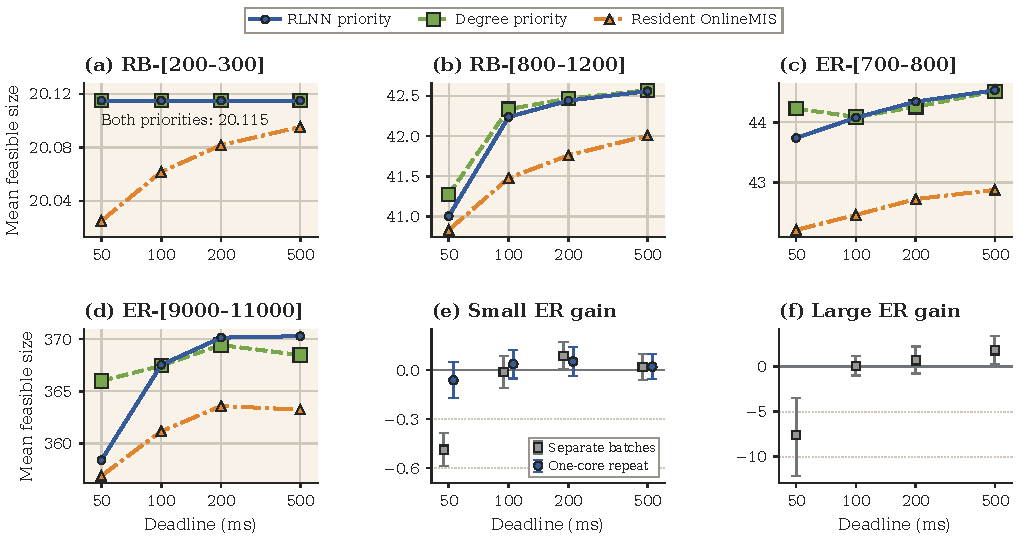
\includegraphics[width=.95\textwidth]{figures/resident_deadlines.pdf}
\caption{\textbf{Delivered size across four independently run deadlines.} (a--d) Mean feasible size at the cutoff over three seeds per graph. There are 1,000 graphs in each RB set, 128 in small ER and 16 in large ER. In (a), blue circles inside green squares mark identical optimal scores. (e--f) Mean size difference between learned and degree ranking on the two ER sets, with pointwise 95\% graph-bootstrap intervals. Panel (e) also shows a repeat interleaving all methods and budgets on one CPU core. Panel legend labels: ``RLNN priority'' is the learned ranking of SPRINT-C and ``Degree priority'' its degree ranking. Table~\ref{tab:resident-details} reports timing and delivery counts.}
\label{fig:resident-curves}
\end{figure*}

SPRINT-C leads resident OnlineMIS in each of the 16 family--budget combinations (Figure~\ref{fig:resident-curves}); the 50~ms large ER difference ($+1.50$, $[-3.19,6.04]$) is the only paired interval that includes zero. On RB-[200--300] SPRINT-C reaches all 3,000 offline-verified optima at every budget with one checkpoint: 375 graphs by a disjoint clique cover and the remaining 625 by an independent SAT check that no larger set exists (Appendix~\ref{app:protocol}). Both rankings attain those optima within 50~ms, at 2.53~ms average return for the degree arm and 10.37~ms for the learned arm; resident OnlineMIS climbs from 2,735 optimal sets at 50~ms to 2,941 at 500~ms. On the 14 register interference graphs the same checkpoint is optimal on all 42 pairs, and the shared greedy initializer reaches the optimum before either ranking is computed (Appendix~\ref{app:gain-sources}).

Figure~\ref{fig:qualitative-instance} follows one instance from release to delivery. The set published before inference already holds 18 vertices; exchanges then trade a held vertex for the candidates it blocks, and the run finishes at 23, one above resident OnlineMIS on the same graph.

Large RB shows why the archive, not the return value, is the quantity a caller can use. At 50~ms all 3,000 runs have a set on the host, yet only 2,525 calls finish before the deadline; at 200~ms resident OnlineMIS also delivers on large RB and small ER, with 190 and 41 calls still running when the budget expires (Table~\ref{tab:resident-details}). Appendix~\ref{app:gain-sources} separates how much of the delivered size comes from constructing and publishing a feasible set and how much from the learned ranking.

\subsection{Execution buys search depth}
On small RB SPRINT-S averages 20.0300 vertices in 193.80~ms, with paired gains of 0.6053 over released RLNN ($[0.5730,0.6387]$) and 0.0793 over RLSA ($[0.0613,0.1003]$) at the 200~ms cutoff (per-pair breakdown in Appendix~\ref{app:representation}, Figure~\ref{fig:baseline-pairs}). Holding the policy fixed, the execution protocol moves the operating point (Table~\ref{tab:policy-path}): with the released weights and 20 particles, fused inference gains 0.5527 vertices over released inference ($[0.5227,0.5847]$); raising the population to 200 adds 0.0587 ($[0.0467,0.0710]$) at the same weights; and the local checkpoint differs from the released one by $-0.0060$ ($[-0.0150,0.0033]$). Execution, not policy training, supplies the gain.

\begin{table}[t]
\caption{Inference protocol, particle count \(K\), and policy weights on the same 3,000 pairs at 200~ms. Steps count parallel updates per trajectory.}
\label{tab:policy-path}
\centering\small
\setlength{\tabcolsep}{3pt}
\begin{tabular}{@{}llrrrr@{}}
\toprule
\paperHeader
\paperHead{Protocol} & \paperHead{Weights} & \paperHead{\(K\)} & \paperHead{Size\,\(\uparrow\)} & \paperHead{Steps} & \paperHead{ms\,\(\downarrow\)} \\
\midrule
Released & Released & 20 & 19.4247 & 85.7 & 152.25 \\
SPRINT-S & Released & 20 & 19.9773 & 1357.9 & 195.84 \\
SPRINT-S & Released & 200 & 20.0360 & 346.2 & 193.87 \\
SPRINT-S & Local & 200 & 20.0300 & 351.0 & 193.80 \\
\bottomrule
\end{tabular}
\end{table}

At 130 steps, replay preserves decoded size at either compilation setting while cutting mean wall time from 277.70 to 74.53~ms (Table~\ref{tab:execution-ablation}). Under a 200~ms deadline the same switches raise search depth from 82.9 to 348.6 steps and add 0.3320 vertices ($[0.3093,0.3563]$); replay supplies 140.0 of the extra steps and compilation another 125.7. Because the fixed-work size is unchanged, the gain is more updates at the same per-step quality, not better updates. Dense adjacency and FP16 follow the same mechanism and add 0.1663 and 0.0493 vertices at fixed time (Appendix~\ref{app:representation}, Figure~\ref{fig:execution-effects}).


\begin{table}[t]
\caption{CUDA Graph replay and policy compilation on matched graph--seed pairs. Entries are means over 3,000 solves per configuration in each protocol.}
\label{tab:execution-ablation}
\centering
\small
\setlength{\tabcolsep}{3pt}
\begin{tabular}{llrrrrr}
\toprule
\paperHeader
 & & \multicolumn{2}{c}{\paperHead{130 steps}} & \multicolumn{3}{c}{\paperHead{200 ms}} \\
\cmidrule(lr){3-4}\cmidrule(lr){5-7}
\paperHeader
\paperHead{Replay} & \paperHead{Compile} & \paperHead{Size\,\(\uparrow\)} & \paperHead{ms\,\(\downarrow\)} & \paperHead{Size\,\(\uparrow\)} & \paperHead{Steps} & \paperHead{ms\,\(\downarrow\)} \\
\midrule
Off & Off & 19.8980 & 277.70 & 19.6967 & 82.9 & 184.07 \\
Off & On  & 19.8930 & 276.31 & 19.6907 & 79.6 & 183.91 \\
On  & Off & 19.8980 & 113.52 & 19.9890 & 222.8 & 192.22 \\
\rowcolor{TableGold}
On  & On  & 19.8930 & \textbf{74.53} & \textbf{20.0287} & \textbf{348.6} & 193.57 \\
\bottomrule
\end{tabular}
\end{table}

\subsection{Delivering earlier at equal size}
At 200~ms, midpoint-plus-terminal and terminal-only decoding both average 20.0303 vertices with full coverage, and their paired size difference is 0.0000 ($[-0.0017,0.0017]$). What changes is when the score exists: midpoint decoding moves the median time to the ultimately scored size from 194.24 to 106.63~ms, and by 125~ms it has published that size on 2,786 of 3,000 pairs, including 2,540 verified optima, where terminal-only decoding has published none. Depths are 351.81 and 353.62 steps and return times 193.55 and 194.03~ms, so the early readout buys availability without paying in quality (Figure~\ref{fig:intro-evidence}(a)). Decoding immediately after initialization costs 0.0187 vertices; Appendix~\ref{app:decode} follows one graph's membership and reports the leading, width and reserve variants.
